\chapter{Data Sources and Methods}\label{sec:methodology}
This chapter lays out the data sources and approach used for the project
\pdfcomment{Explain how my processing chain differs from the NASA one}
\pdfcomment{mention the UTM grid reprojection steps if they're not mentioned.}
\section{Data Sources}
The following data sources were used as input to the processing chain
\subsection{NASA ATL03 global geolocated photon data}

The main source of data is NASA's ATL03 V005 data product \parencite{icesat2data}. ATL03 is a level 1 data product that consists of the precise latitude, longitude, and elevation for each received photon. As a level 1 data product, it has already undergone some processing by the Atlas Science Algorithm Software (ASAS) to correct for instrument errors, to classify photons as likely signal or noise for different surface types, and to correct for some geophysical effects including earth tides to provide provide measurements relative to the WGS-84 ellipsoid. 

Additionally, the data includes variables that allow for further corrections and adjustments to the tide-free geoid reference system. These additional variables include correction factors for the tide, ocean surface depression due to atmospheric pressure, and factors to convert the ellipsoidal elevation to a height relative to the tide-free geoid.

\subsection{GEBCO Global Grid 2021}

The General Bathymetric Chart of the Ocean (GEBCO) is a global grid of topography and bathymetry at a 30 arc-second mesh resolution \parencite{gebco2021griddata}. GEBCO is assembled by compiling many different data sources, including mutli-beam sonar data, nautical charts, and satellite gravimetric measurements for deep-ocean bathymetry \parencite{gebcocookbook}. The elevation data is referenced to a vaguely-defined 'mean sea level'. The various data sets included in GEBCO are all assumed to be referenced to MSL, but some datasets referenced to chart datum are included. 

GEBCO has a limited accuracy and resolution, but it is the only available data source in many places in the world, so it is sometimes used as the best-estimate in very data-poor sites. However, the accuracy of GEBCO varies depending on the input data sources. In this project, the GEBCO elevation is used both to filter locations that \emph{may} contain valid bathymetry, and used as a prior guess to the bayesian updating approach. 

\subsection{GlobColour Daily Secchi Disk Depth Data}

To investigate the relationship between the water clarity and the availablity and quality of the bathymetric data from the spaceborne lidar, data from \citeauthor{Garnesson2019} is also linked to each transect to investigate the relationship between the Secchi Disk Depth along the transect. The exact data product used is \cite{Garnesson2019}. The data is accessed via the OPeNDAP protocol hosted by the Copernicus Marine Service, using the Xarray python package \parencite{hoyer_stephan_2022_6323468,hoyer2017xarray}.



\section{Methodology}


To reach the end goal of incorporating ICESat-2 into GEBCO grids, first the lidar photon data for the area of interest is downloaded, processed into geoidal heights, subset to only include subsurface photons, find bathymetric signal within the subsurface data, interpolate into a 2D grid, then finally combine the interpolated ICESat-2 data with the resampled GEBCO grid within the area of interest. Then, for the test sites, the change in in the various error metrics between the naive bilinear interpolation is calculated. 


\begin{figure}[h]
    \centering
    \import{figures/drawio}{Methodology_overview.drawio.svg.pdf_tex}
    \caption{Overview of the basic methodology}
    \label{fig:methodology-overview}
\end{figure}

\subsection{Processing ATL03}
To download data for a specific site geographic area of interest is created, and this area is passed to the NSIDC download API to use for spatial subsetting. This allows spatial subsetting of the data download which reduces file size. The NSIDC API also allows subsetting by the variable name, so only the ATL03 variables that are relevant for this research are downloaded, which further reduces the file size for practical download and storage of the ATL03 data. 

The three variables that define the 3D location in the WGS-84 reference frame of each photon are \emph{h\_ph}, \emph{lat\_ph}, and \emph{lon\_ph} are located in the \emph{heights} group within the ATL03 data structure. To use these variables for the purpose of bathymetric measurement, several other variables are required for processing. To transform the ellipsoidal elevation to the geoidal elevation, the two additive factors \emph{geoid} and \emph{geoid\_free2mean} are included in the download.

These correction factors are not provided for every photon but are provided for each 20m segment because they vary at scales longer than the nominal 0.7m between each photon. To find the correct adjustments factors for each photon, we need to match the segment-rate variables to the photon rate variables. This is done using the python package Pandas \parencite{jeff_reback_2022_6408044,mckinney-proc-scipy-2010} which has functions for joining time series data.  The segment-rate variable for each photon is determined using the Pandas dataframe \emph{asof()} method to find the closest segment rate variables in time to each photon. 

\begin{figure}[h]
    \centering
    \includegraphics[width=0.75\textwidth]{figures/reference_photon_plot.pdf}
    \caption{Relation between the regular photons, and the 20m segment rate variables}
    \label{fig:reference-photon_match} 
\end{figure}

\subsection{Filtering ATL03 to subsurface returns}

The bathymetric signal that we are seeking to find is located in the shallow-water nearshore zone. Therefore, photons outside that zone need to be removed reduce processing time and eliminate false positives as much as possible. To reduce the downloaded transect data within the area of interest, the following filtering steps are applied to each transect \pdfcomment{Add figures For each of these steps}:

\begin{enumerate}
    \item For every photon, find the GEBCO depth at that location. Any photons with a GEBCO elevation between -50 and 3m are selected, and those outside of this region are culled from the data set. Points that are outside this range are assumed to be deeper than the maximum known depth detectable by ICESat-2 (38m per \citeauthor{Parrish2019}), or assumed to be on land. This provides a horizontal filtering along the transect. An example of this process can be seen in figure \ref{fig:gebco_filtering}
    
    \begin{figure}[h]
        \centering
        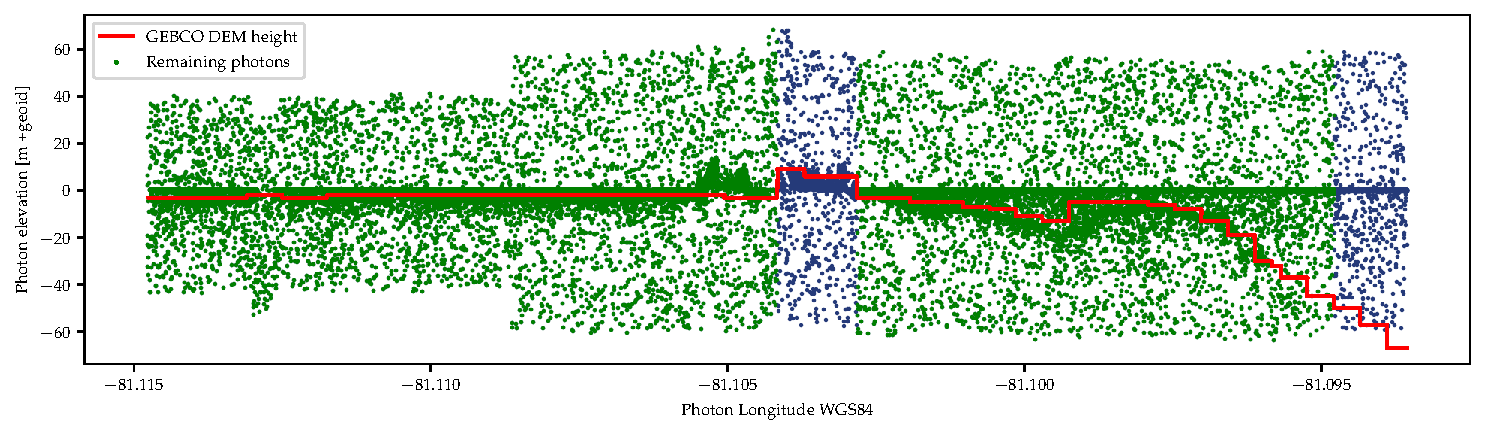
\includegraphics[width=\textwidth]{figures/methodology_gebco_filtering.pdf}
        \caption{The GEBCO data for the example transect, and the photons that are removed due to the GEBCO depth}
        \label{fig:gebco_filtering}
    \end{figure}

    \item To remove any high noise, cloud returns, or any remaining high land points not removed in step 1, any points more than 5m above the geoid are removed, based on the approach in \citeauthor{Ranndal2021}.
    \item The local sea-surface elevation $h_{sea}$ is calculated by taking the median elevation of photons that are classified as high-confidence sea surface photons. The water depth for each photon is then calculated. The standard deviation of the elevation high-confidence photons $\sigma_{h_{sea}}$ is also calculated to estimate the magnitude of the wave height at the time of the observation.
    \item Any points with a water depth greater than 40 meters, and points with an geoidal height  less than -40m are removed, based on the same assumption that they are too deep to be bathymetric points. 
    \item Any points that are higher than $h_{sea} + max(\sigma_{h_{sea}},1)$ are removed. 
    
    
    The results of steps 3-5 are shown in figure \ref{fig:vert_filtering}
    % TODO fix this graph legend
    \begin{figure}[h]
        \centering
        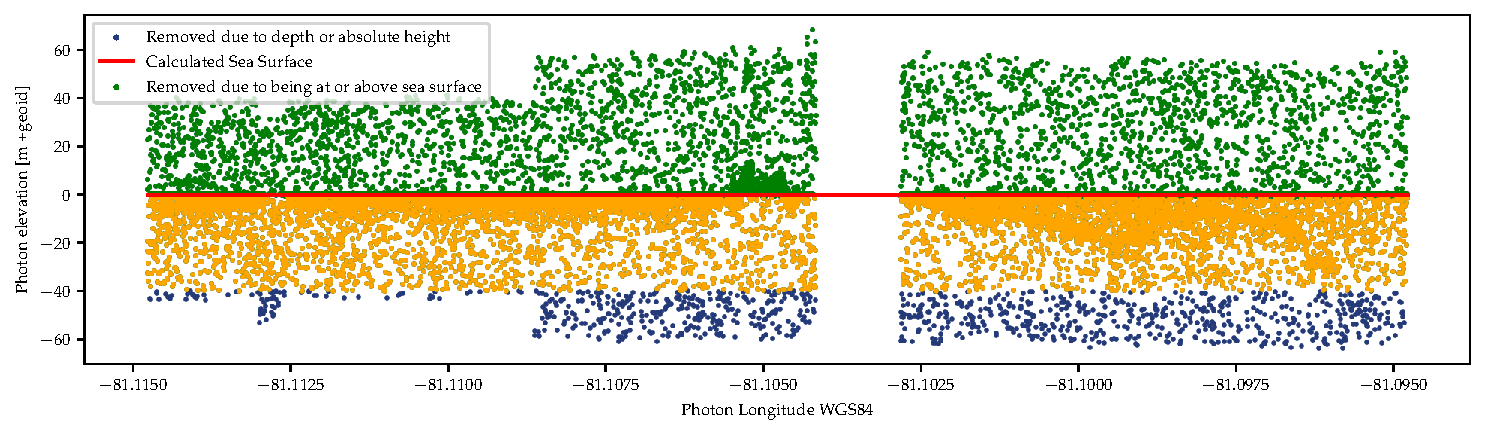
\includegraphics[width=\textwidth]{figures/methodology_sealvl_filtering.pdf}
        \caption{Vertical point filtering based on the local sea surface elevation}
        \label{fig:vert_filtering}
    \end{figure}
\end{enumerate}

After these filtering steps, the resulting subsurface photons for this example transect are shown in figure \ref{fig:remaing_photons}. The bathymetric signal can be seen clearly throughout the entire transect.

\begin{figure}[h]
    \centering
    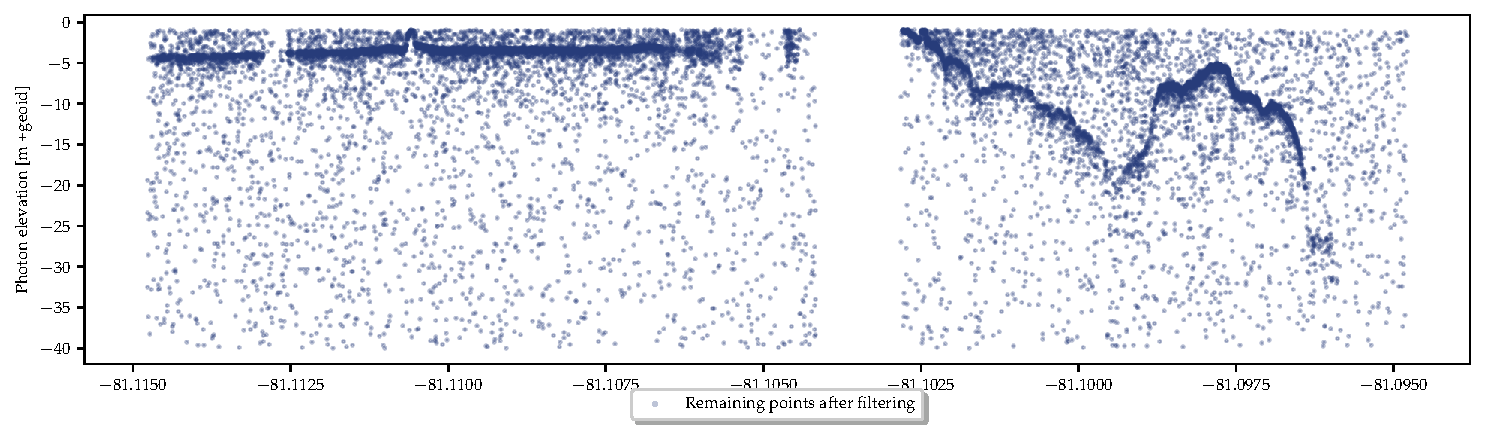
\includegraphics[width=\textwidth]{figures/methodology_reminaing_after_filtering.pdf}
    \caption{Subsurface photons found resulting after the filtering process}
    \label{fig:remaing_photons}
\end{figure}

An overview of the entire filtering chain is shown in figure \ref{fig:filtering-flowchart}

\begin{figure}[h]
    \centering
    \import{figures/drawio}{Filtering_algo.drawio.svg.pdf_tex}
    % \import{figures/drawio}{filtering_v2.drawio.svg.pdf_tex}
    \caption{Filtering Process}\pdfcomment{figure out the word wrap issue}
    \label{fig:filtering-flowchart}
\end{figure}

Finally, before the signal-finding is applied, the Parrish method of refraction correction is applied to all subsurface photons.

\begin{figure}[htbp]
    \centering
    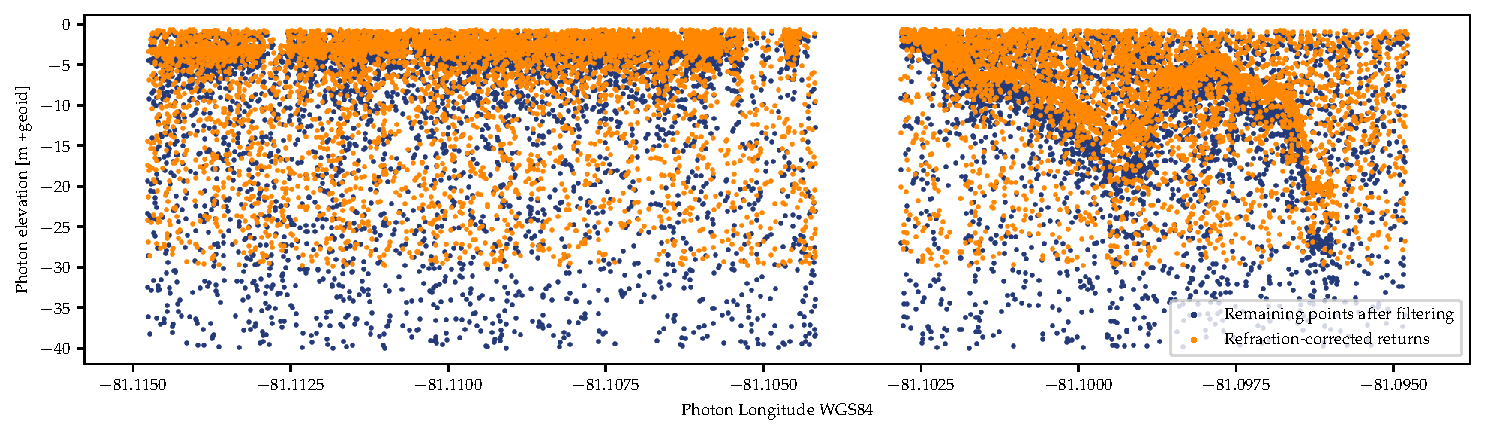
\includegraphics[width=\textwidth]{figures/methodology_refraction.pdf}
    \caption{The refraction correction applied to the remaining photons}
    \label{fig:refraction-photons}
\end{figure}

\subsection{Bathymetric Signal Extraction}\label{sec:kdesignalfinding}

The filtering steps reduce the dataset to just photon that are in the subsurface zone. To determine if there is bathymetric signal present, further processing is required. Some proposed methods for separating bathymetric signal photons from noise are explained in section \ref{subsec:denoising}. For this project, a new method is proposed based on a Gaussian Kernel Density Estimation (KDE) function. A function is created that returns the maximum kernel density, and the Z location at which it occurs. $$ f(\hat{z}_{window}) \rightarrow kde_{max},z_{kde_{max}} $$ Figure \ref{fig:kdefunc} shows the KDE function as applied to an example window, and the resulting kernel density plot. The KDE function is highly influenced by the \emph{bandwidth} parameter. For this implementation, the Scott method \parencite{Scott2015} is used to estimate the required bandwidth based on the distribution of the data. 

This function is applied on a rolling basis to a window of 100 adjacent photons. This function returns a value for every single point along the transect, including in areas that do not have any noticeable signal. The kernel density value gives an indication of the strength of the peak. To reject the locations where the signal is weak, any points with a KDE value of less than the median value $$ kde_{50} $$  are assigned an NaN value and are dropped from the analysis.

\begin{figure}[htbp]
    \centering
    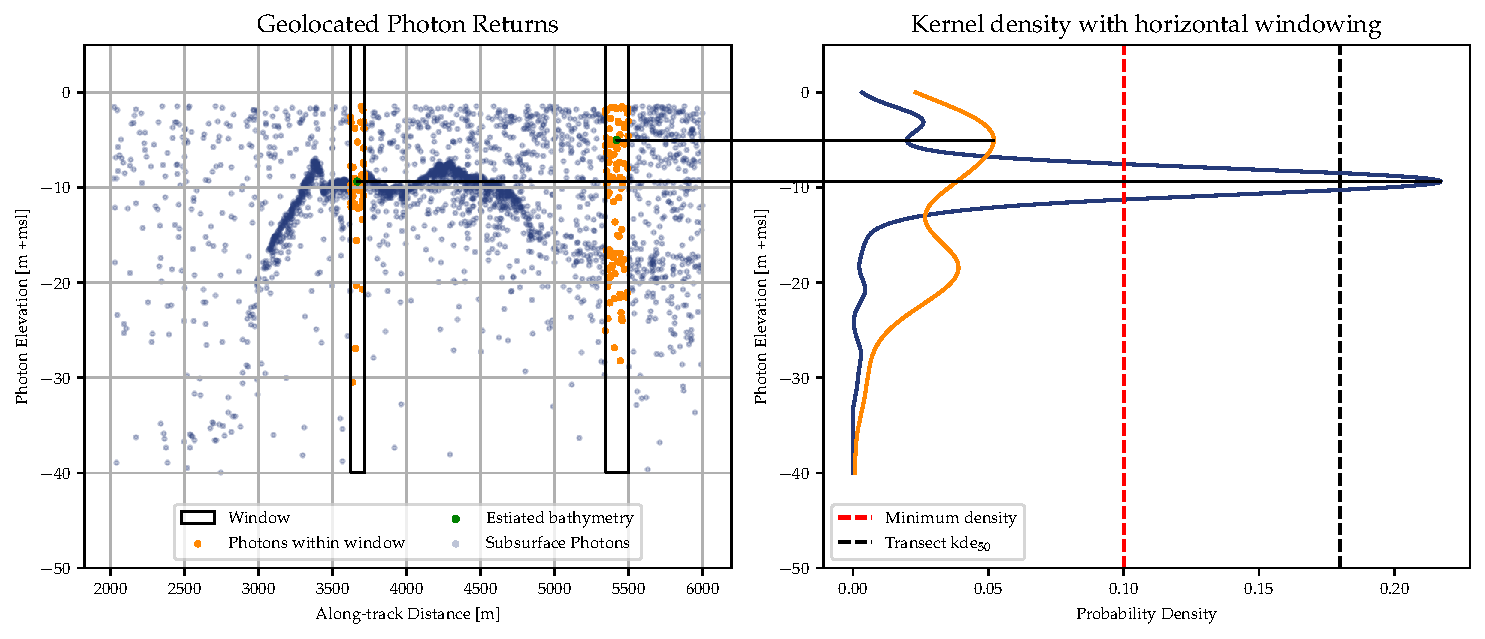
\includegraphics[width=\textwidth]{figures/2d_kde_plot.pdf}
    \caption{KDE function as applied to single window}
    \label{fig:kdefunc}
\end{figure}

The input parameters to the signal finding function are:

\begin{enumerate}
    \item The size of the window in \emph{number of points}
    \item the cutoff value for the Kernel Density required for point to be considered signal
\end{enumerate}

\subsection{Interpolation to a 2D grid}

After the bathymetric signal points are identified per the method in \ref{sec:kdesignalfinding}, the resulting bathymetry points are densely spaced along satellite tracklines, but are absent between them. A number of interpolation techniques have been applied to create bathymetry grids from point data. Commonly, inverse-distance weighting (IDW), tension splines, or loess interpolators have been used \parencite{gebcocookbook,Ferreira2017}. These approaches are relatively straightforward and easy to implement. However, the disadvantage of these simple approaches that there is not a clear methodology of establishing the uncertainty of the resulting interpolation. Intuitively, areas with a higher point density will lead to a interpolation with a lower uncertainty that areas with very sparse points. Kriging is a geostatistical technique that allows interpolating points into a grid, while also giving an indication of the uncertainty in the neighborhood. By knowing both our estimated sea floor depth and the uncertainty in the estimate, we can use a bayesian approach to update our initial guess of the seafloor location.


\subsubsection{Subsampling of Bathymetric points using Poisson Disk Sampling} \pdfcomment{maybe add a figure to show the process better} \label{subsec:poissonsubsampling}
The bathymetric points are extremely densely spaced in some areas and transects. This can present an issue to kriging, which is computationally expensive and points too close together can make the algorithm even slower. To reduce the number of points fed into the algorithm, a subsample of the points is taken using the Poisson disk sampling technique. Poisson disk sampling is a strategy that generates random samples of a distribution that are a minimum distance apart. When applied to a point cloud, in this case the point cloud of all the bathymetric points, the sampling function will only return points that are a minimum distance apart in 3d space. This ensures that the sampling is as representative as possible of the underlying surface.

The implementation used is from the PDAL software library \parencite{howard_butler_2022_6369164}, which provides an iterative Poisson disk sampling function based on \citeauthor{McCool1992}. The disk sampling is applied iteratively with a decreasing radius until the desired number of points is reached. In this case, it was found that the maximum number of points that can be practically be used is approximately 2000 points. Therefore, this was the number of points used to allow the maximum possible point density while using consumer-grade laptops to run the algorithm. 

\subsubsection{Kriging interpolation}
Using the subsample of the points from the poisson disk sampling, they are converted to a bathymetry raster using universal kriging. This geostatistical technique results in both a raster of the estimated depth as well as the estimated uncertainty. The python package Pykrige \parencite{benjamin_murphy_2021_5380342} was used to implement the universal kriging approach. \pdfcomment{add variogram parameter discussion}


\subsection{Bayesian data assimilation using kalman update equation}
The Kalman Filter is a mathematical technique to predict the state of systems based on uncertain measurements. It consist of a loop of two steps, an \emph{time update} step which updates the position based on a measurement and a known measurement uncertainty, and a \emph{measurement update} step which predicts the state based on the dynamic equations of the system. The Kalman filter equations, for a state $x_k$ and a vector of measurements of the state $z_k$:

Time Update:

\begin{equation}
    \hat{x}_{\bar{k}} = A\hat{x}_{k-1} + B\hat{u_{k-1}}
\end{equation}

\begin{equation}
    P_{\bar{k}} = A P_{k-1} A^T + Q
\end{equation}

Measurement Update:
\begin{equation}
    K = P_{\bar{k}} H^T(H P_{\bar{k}} H^T + R) ^{-1}
\end{equation}

\begin{equation}
    \hat{x}_k = \hat{x}_{\bar{k}} + K(\hat{z}_k - H \hat{x}_{\bar{k}})
\end{equation}

\begin{equation}
    P_k = (I - KH)P_{\bar{k}}
\end{equation}


The coastal zone is a highly dynamic system. However, for the purposes of this project is is assumed that the temporal variations over the time scale being studied are within the margin of error of the measurements, so the bathymetry of the nearshore zone is assumed to be a static system and the time update step can be ignored. It is also assumed all measurements are measurements of the same underlying physical depth, and that differences between measurements are due to normally distributed measurement error, with magnitude of the error varying depending on the method. To combine multiple measurements, the \emph{measurement update} step is applied recursively for each available measurement, producing a bayesian estimate of the bathymetry, in that it considers the uncertainty of each estimate. 

\subsection{Error Evaluation}

There are two different types of error being evaluated to test the results of the different parts of the method. Both the error between the validation data and the lidar data is checked to evaluate the performance of ICESat-2 measurements, and the signal finding algorithm, and the total decrease in error between GEBCO and the version of GEBCO that includes the interpolated ICESat-2 data. 

The error metrics that are evaluated for both types of error are the root mean square error (RMSE) and the mean absolute error (MAE). The RMSE is calculated by takign the mean of the squared difference between the true value and the estimated value, and then taking the square root of this mean.

$$  RMSE = \sqrt{\frac{1}{n}\Sigma_{i=1}^{n}{\Big(\frac{d_i -f_i}{\sigma_i}\Big)^2}}  $$

By squaring the error first, larger magnitude errors are given relatively more weight in the metric. Mean absolute error also gives an idea of the average deviation, but gives equal weight to all errors.

$$ MAE = \sum_{i=1}^{D}|x_i-y_i| $$

To evaluate these errors between the kalman-updated bathymetry grid and the validation data. Reprojection and resampling is required. The validation data has a horizontal resolution on the order of 1m, while GEBCO has a horizontal resolution on the order of 450m. Before taking the error, the data being compared is first reprojected into the native coordinate system and resolution of the validation data using GDAL \parencite{rouault_even_2022_6352176}. Then, the RMSE and MAE can be calculated between each cell of the raster grid.

\pdfcomment{make add figures showing the grid resampling/reprojection steps}

% \subsection{Evaluating transect-level variables which predict bathymetry}
% \pdfcomment{This could potentially be interesting and also help flesh out my answer to my first research question}
